\section{Impact on T2K Oscillation Analyses}
The parameter set from the data fit is now used to gauge the impact on the oscillated $E_{rec}$ spectrum at SK. The high dimensional posterior distribution sampled by the MCMC after burn-in, containing 50 flux and 23 interaction parameters, is propagated without assumptions on the shape of the probability distribution function.

Using the oscillation parameters in \autoref{tab:osc_pars}, the posterior predictive distribution is formed by taking 10,000 random draws from the ND280-only MCMC to data, presented in \autoref{sec:datafit}. The oscillation parameters and SK detector parameters are fixed to their prior values and are not varied.
\begin{table}[h]
	\begin{tabular}{l | c}
		\hline
		\hline
		Parameter & Value \\
		\hline
		$\sin^2\theta_{12}$ & 0.304 \\
		$\sin^2\theta_{23}$ & 0.528 \\
		$\sin^2\theta_{13}$ & 0.0219 \\
		$\Delta m^2_{12}$  & $7.53\times10^{-5} \text{ eV}^2$ \\
		$\Delta m^2_{23}$  & $2.509\times10^{-3} \text{ eV}^2$ \\
		$\delta_{cp}$ & -1.601 \\
		\hline
		POT FHC & $1.47341\times10^{21}$ (runs 2 to 8)\\ 
		POT RHC & $7.5573\times10^{20}$ (runs 2 to 8)\\
		\hline
		\hline
	\end{tabular}
\caption{Oscillation parameters used to produce nominal event rates at SK}
\label{tab:osc_pars}
\end{table}

The integrated event rates is shown in \autoref{tab:sk_evt_rates_2017}. As for the ND280 event rates in \autoref{tab:postfit_eventrate}, the impact of the ND280 posterior compared to the prior is dramatic, reducing uncertainty by 60-80\% for all SK selections.
% from /tmp/ts-out.2tydjK on heppc105, June 1, 10,000 throws
\begin{table}[h]
	\begin{tabular}{l | c c | c c}
		\hline
		\hline
		Sample & \multicolumn{2}{c|}{Event rate} & \multicolumn{2}{c}{$\delta N/N$ (\%)} \\
		& Pre-fit & Post-fit & Pre-fit & Post-fit \\
		\hline
		$1\text{R}\mu$ & $249.86\pm34.96$ & $262.59\pm8.03$ & 13.99 & 3.06 \\
		$1\text{R}e$ & $65.62\pm9.95$ & $72.13\pm2.88$ & 15.16 &  3.99   \\
		$1\text{R}e \text{ 1d}e$ & $7.70\pm0.93$ & $6.73\pm0.32$ & 12.08 & 4.75  \\
		
		$1\text{R}\mu \text{ RHC}$ & $61.50\pm7.21$ & $62.57\pm1.73$ & 11.72 & 2.76 \\
		$1\text{R}e \text{ RHC}$ & $7.64\pm0.95$ & $7.72\pm0.32$ & 12.43 & 4.15  \\
		\hline
		\hline
	\end{tabular}
\caption{T2K-SK event rates and uncertainties from flux and interaction systematics with and without near-detector constraints from this analysis (not including SK and oscillation parameter errors)}
\label{tab:sk_evt_rates_2017}
\end{table}

The $E_{rec}$ spectrum using the prior and posterior distributions for each SK selection is shown in \autoref{fig:sk_2017}. The $1\text{R}\mu$ distributions are consistent for FHC and RHC , in which there is an enhancement at low $E_{rec}$ up until the oscillation dip, followed by a prediction much in agreement with the prior after $E_{rec}\sim0.6\text{ GeV}$. This impacts $\Delta m^2$ and $\sin^2\theta_{23}$, since both the depth and slope of the dip changes. 

The fit has little effect on the central value of the $1\text{R}e$ RHC selection but reduces the uncertainty by more than 50\% above the oscillation dip. The two FHC $1\text{R}e$ selections show opposite behaviour: $1\text{R}e$ is enhanced throughout the spectrum, sitting approximately on the $1\sigma$ of the uncertainty band of the prior, with increasing agreement with the prior with increasing $E_{rec}$. The 1d$e$ selection is instead reduced throughout $E_{rec}$, largely due to the ND280 1$\pi$ selections being overestimated when using the prior values.
\begin{figure}[h]
	\begin{subfigure}[t]{0.32\textwidth}
		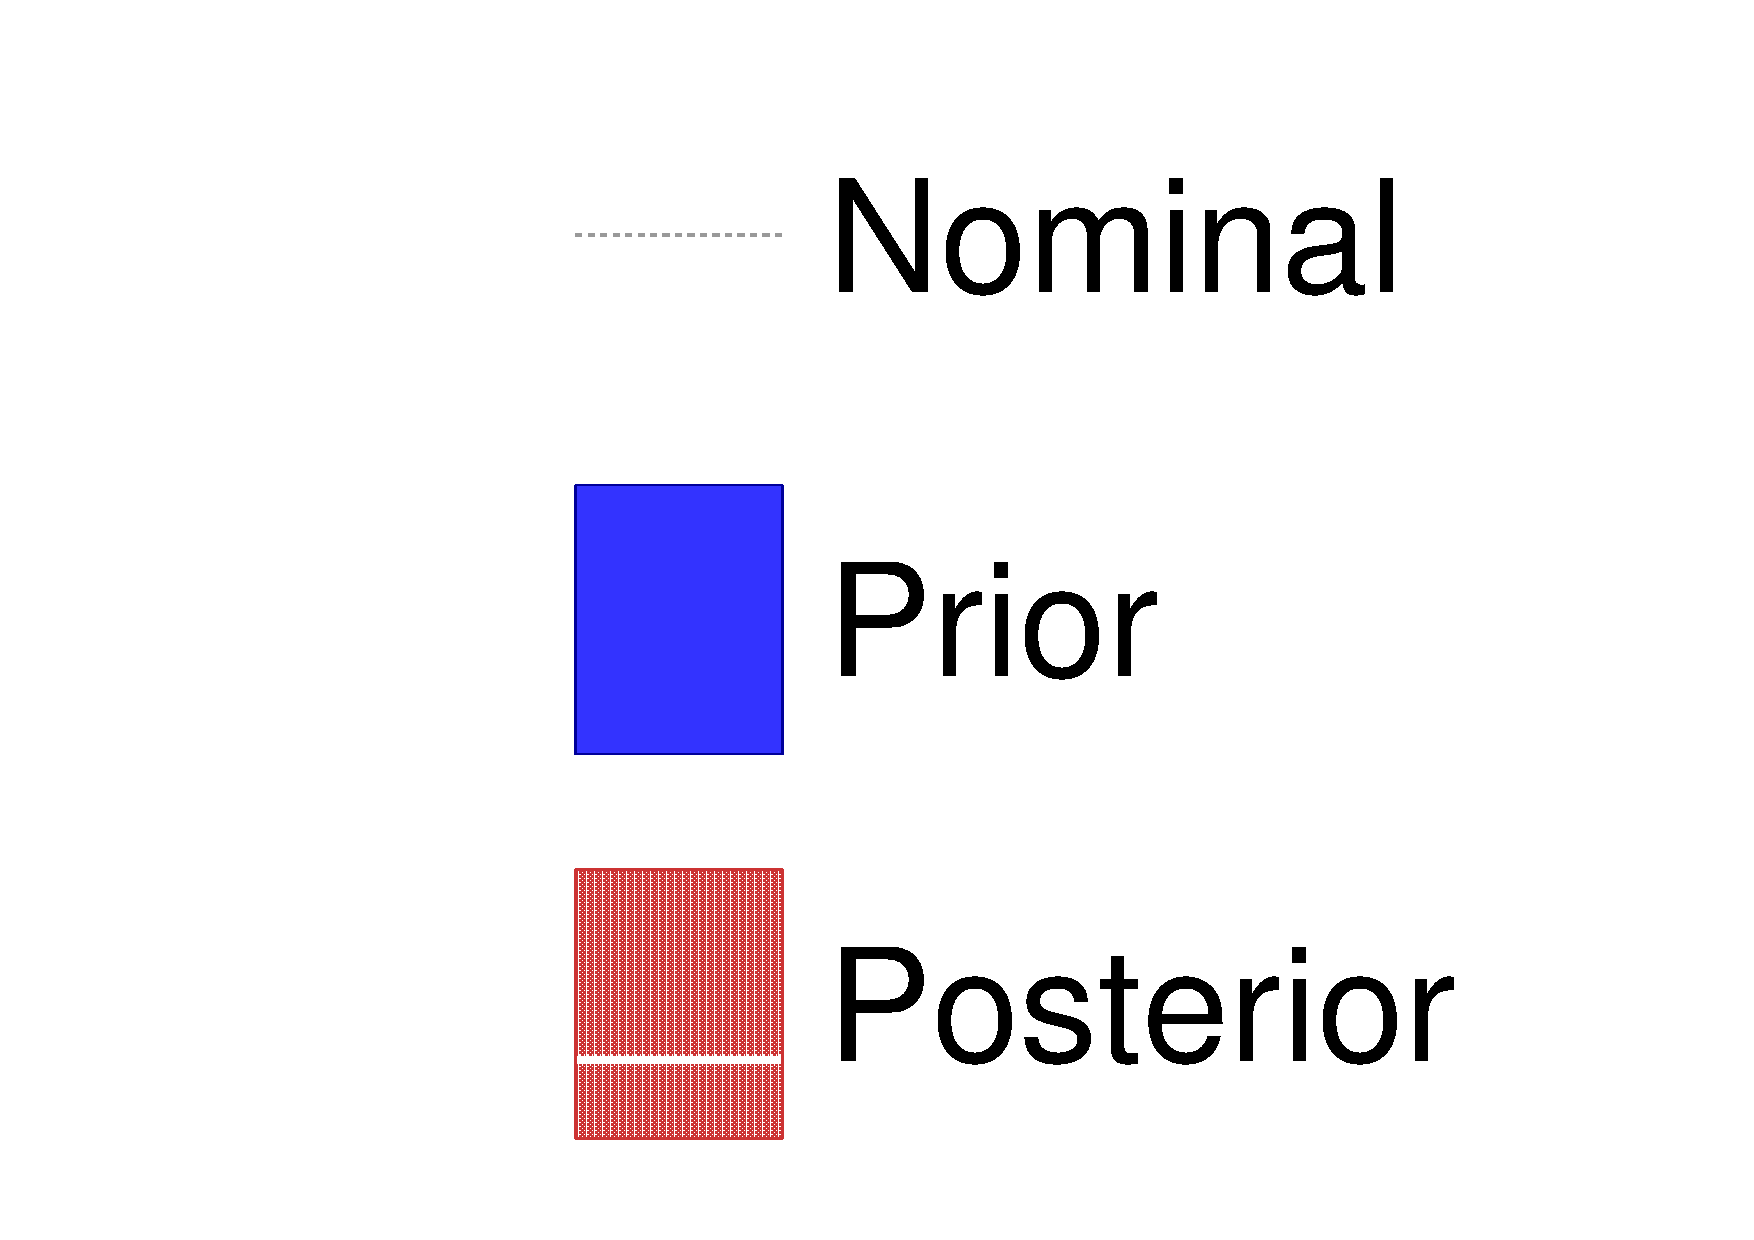
\includegraphics[width=\textwidth, trim={0mm 0mm 0mm 0mm}, clip, page=1]{figures/mach3/data/prior_error_1june_try_2017_fit_on_sk_spectra}
	\end{subfigure}
	\begin{subfigure}[t]{0.32\textwidth}
		\includegraphics[width=\textwidth, trim={0mm 0mm 0mm 0mm}, clip, page=5]{figures/mach3/data/prior_error_1june_try_2017_fit_on_sk_spectra}
	\end{subfigure}
	\begin{subfigure}[t]{0.32\textwidth}
		\includegraphics[width=\textwidth, trim={0mm 0mm 0mm 0mm}, clip, page=6]{figures/mach3/data/prior_error_1june_try_2017_fit_on_sk_spectra}
	\end{subfigure}
	
	\begin{subfigure}[t]{0.32\textwidth}
		\includegraphics[width=\textwidth, trim={0mm 0mm 0mm 0mm}, clip, page=2]{figures/mach3/data/prior_error_1june_try_2017_fit_on_sk_spectra}
	\end{subfigure}
	\begin{subfigure}[t]{0.32\textwidth}
		\includegraphics[width=\textwidth, trim={0mm 0mm 0mm 0mm}, clip, page=3]{figures/mach3/data/prior_error_1june_try_2017_fit_on_sk_spectra}
	\end{subfigure}
	\begin{subfigure}[t]{0.32\textwidth}
		\includegraphics[width=\textwidth, trim={0mm 0mm 0mm 0mm}, clip, page=4]{figures/mach3/data/prior_error_1june_try_2017_fit_on_sk_spectra}
	\end{subfigure}
	
	\caption{Impact of the full fit on SK spectra compared to the prior}
	\label{fig:sk_2017}
\end{figure}

The impact of the alternate studies mentioned earlier and their impact on the SK prediction are detailed in \autoref{sec:data_alt_studies}.